\section{The Price of Stability of Approximate Nash Equilibria}\label{sec:bicriteria}

So our task is to compare the social welfare of the best $\epsilon$-Nash equilibrium with
the social welfare of the optimal solution. Let's begin by investigating the optimal solution.

\subsection{An Optimal Delegation Graph} 
By the linearity of expectation, there is an optimal solution in which the agents use only pure strategies. 
In particular, there exists an {\em optimal} delegation graph maximizing social welfare. Moreover, this optimal graph 
has interesting structural properties. 
To explain this, we say that agent $i$ is {\em happy} if she has strictly positive utility in a delegation graph $G$, that is 
$u_{i,g(i)}>0$.  A component $Q$ in $G$ is {\em jolly} if every vertex in $Q$ (except, possibly, the guru) is happy.

The key observation then is that there is an optimal delegation graph in which every component is a jolly star. 

 
\begin{lem}\label{lem: OptLD}
There is an optimal delegation graph that is the disjoint union of jolly stars.
\end{lem}
\begin{proof}
Let $Q$ be a component in an optimal delegation graph $G$. We may assume $Q$ contains a guru.
To see this, suppose $Q$ contains an abstaining sink node $j$. Then the graph $\hat{G}=G\cup (j,j)$ where $j$ votes 
herself is also optimal. On the other hand, suppose $Q$ contains a cycle $C$ of length at least $2$. Take an agent $j\in C$. 
Then the graph $\hat{G}$ obtained by $j$ voting herself instead of delegating her vote is also optimal.

So we may assume each component contains a guru. Further, we may assume each component is a star.
Suppose not, take a component $Q$ with guru $j$ containing an agent $i$ that does not delegate to $j$.
But then the graph $\hat{G}$ obtained by $i$ delegating her vote directly to $j$ is optimal.

Finally, we may assume each star is {\em jolly}. Suppose $i$ is not a happy agent in a star $Q$ with guru $j$.
Thus $u_{ij}=0$. But then if $i$ changes her delegation and votes herself we again obtain an optimal solution.
In this case $i$ will form a new singleton component which is trivially a jolly star. \qed
\end{proof}

Lemma~\ref{lem: OptLD} states that the optimal solution can be obtained by a pure strategy~$\x^{*}$ whose 
delegation graph is union of jolly stars. The centre of each star is a guru in the optimal solution and the leaves are the 
corresponding happy agents who delegated to the guru.  Denote the set of gurus in the optimal solution by $D^{*}=\{i\in V \ : \ x^*_{ii}=1\}$,  
and let $L_j = \{i\in V\setminus D^{*} \ : \ x^*_{ij}=1\}$ be the agents who delegate to the guru $j$ as illustrated in Figure~\ref{Fig: Star}. It follows that the optimal solution has welfare
$$
\Opt = \sum_{j\in D^{*} } \left( u_{jj} + \sum_{i\in L_j}u_{ij}\right)  
$$ 

\begin{figure}[bt!]
	\centering
	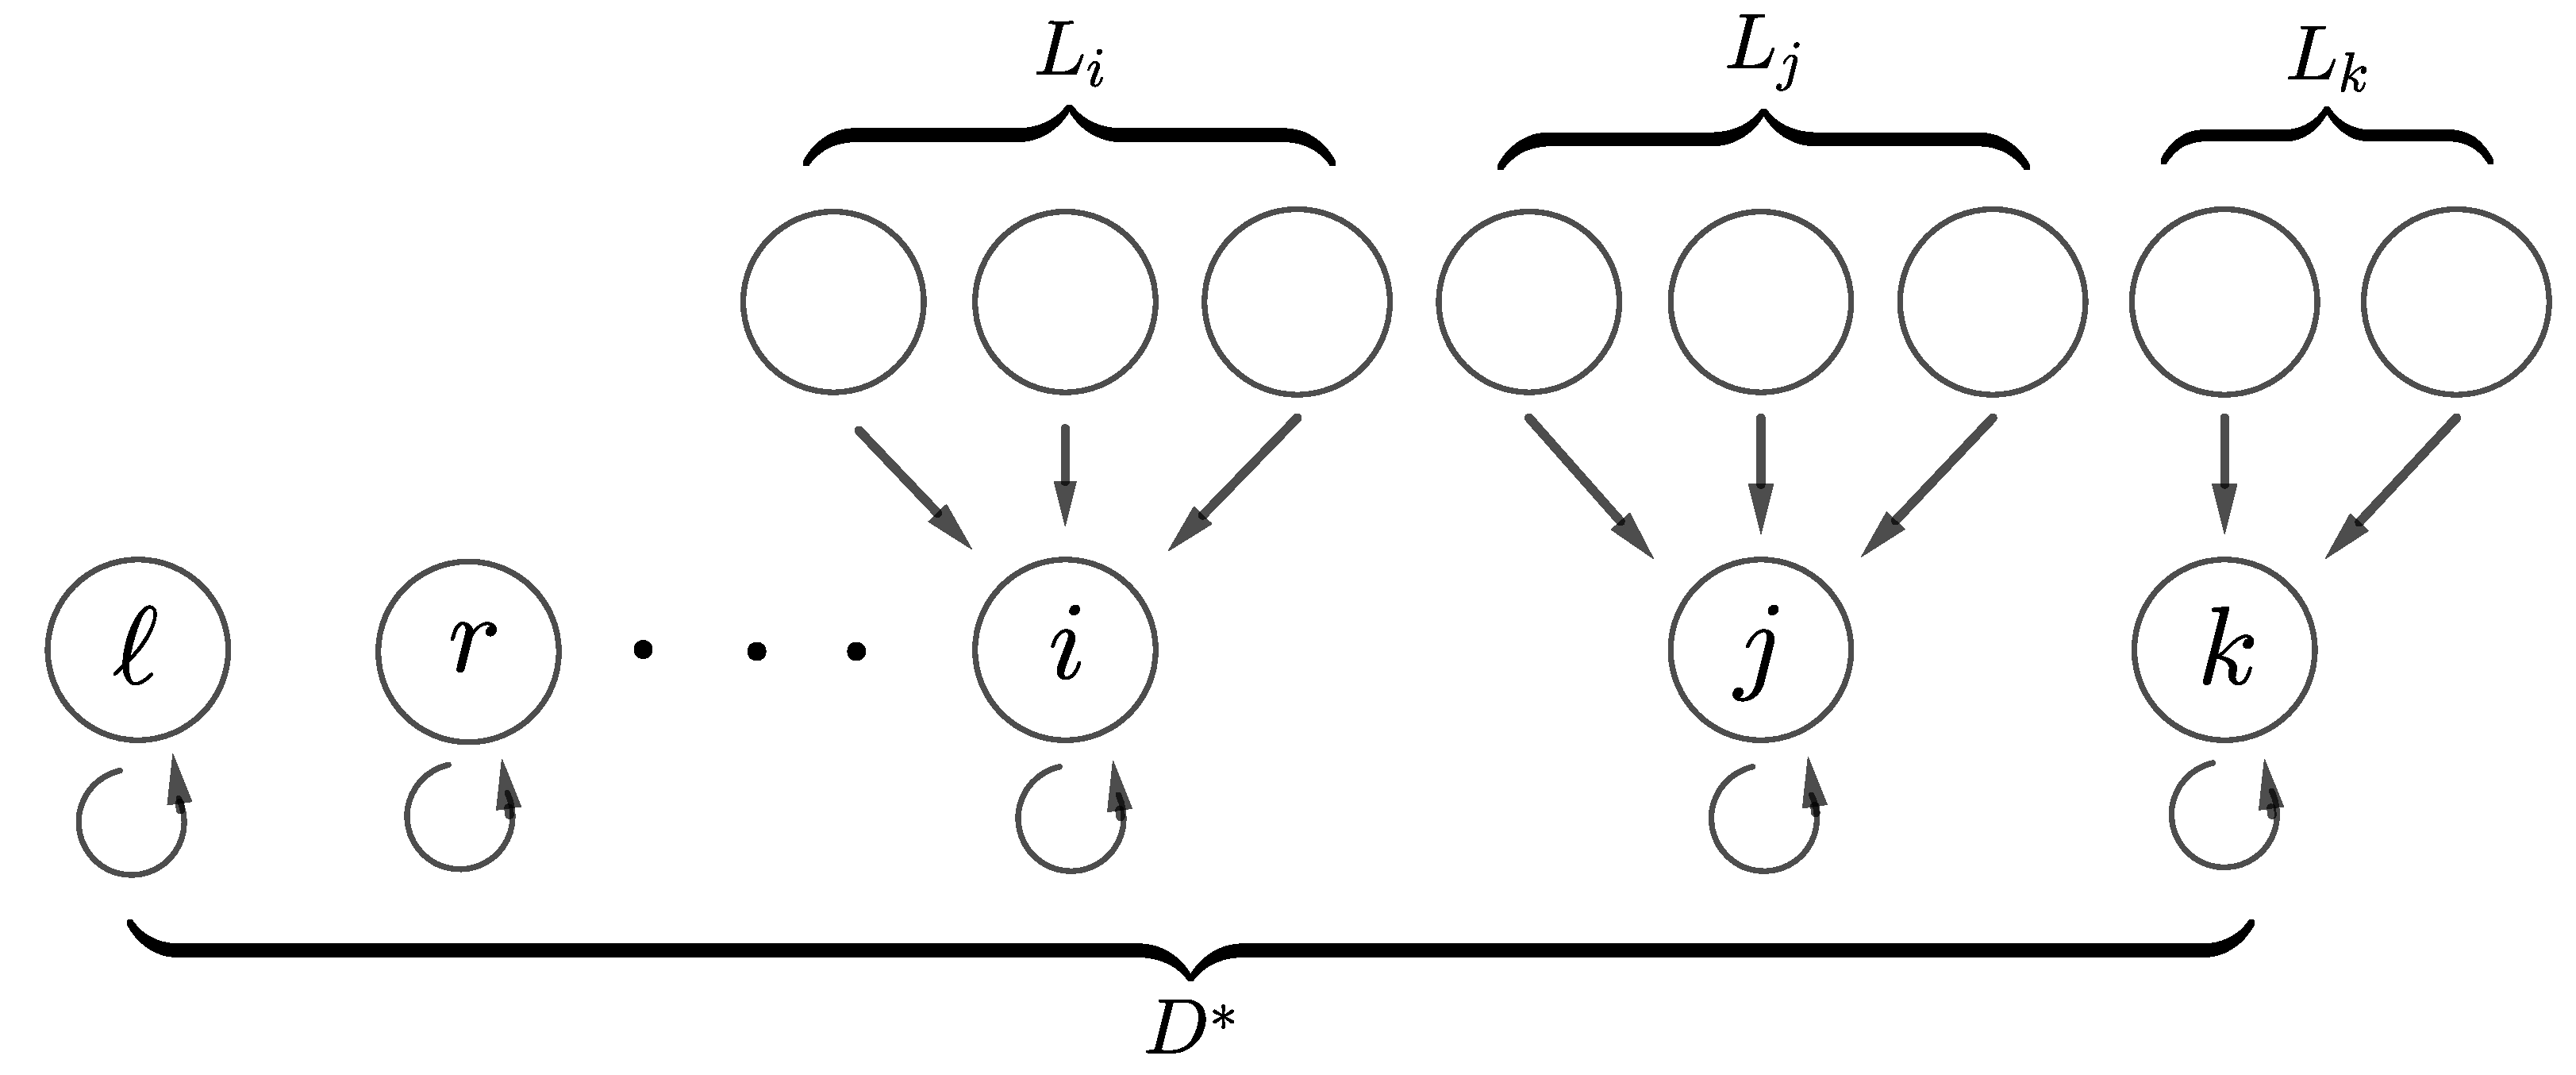
\includegraphics[scale=0.14]{Star}
	\caption{Welfare optimal delegation graph that is disjoint union of jolly stars. }
	\label{Fig: Star}
\end{figure}
\subsection{A Stable Solution}

In order to study the best $\epsilon$-Nash equilibrium we now show the existence of
a ``potentially'' stable solution $\x$ whose definition is inspired by the set $D^*$ of gurus in the optimal solution. 
In Section~\ref{sec:bounds} we will prove that $\x$ is indeed an $\epsilon$-Nash equilibrium and also has high
social welfare.

To obtain $\x$ we require the following definitions.
Denote the standard set of feasible mixed strategies for agent $i$ as 
$$\mathbb{S}_i=\{ \x_{i}\in \mathbb{R}^n_+ \ : \ \sum\limits_{j\in V}x_{ij}=1\  \}$$
Given a fixed strategy profile $\x_{-i}=\{\x_j\}_{j\neq i}$ for the other agents, let
the corresponding best response for agent $i$ be 
$$B_i(\x_{-i})=\argmax\limits_{\hat{\x}\in \mathbb{S}_i} u_{i}(\hat{\x},\x_{-i})$$
For each $i\in D^*$, we denote a restricted set of mixed strategies 
$$\mathbb{S}^R_i = \{ \x_{i}\in \mathbb{R}^n_+ \ : \ \sum\limits_{j\in V}x_{ij}=1\ , x_{ii}\geq \epsilon \}$$
Then for a fixed strategy profile $\x_{-i}$, let 
$$B^{R}_i(\x_{-i})=\argmax\limits_{\hat{\x}\in \mathbb{S}^R_i } u_{i}(\hat{\x},\x_{-i})$$ 
be the best response for the agent $i$ from amongst the restricted set of feasible strategies. 
Next recall Kakutani's Fixed Point Theorem.
\begin{thm}[Kakutani's Fixed Point Theorem] 
Let $K$ be a non-empty, compact and convex subset of $\mathbb{R}^m$, and let $\Phi:K \rightarrow 2^K$ be a set-valued 
function on~$K$ such that:\\
\indent (i) $\Phi(x)$ is non-empty and convex for all $x\in K$, and\\
\indent (ii) $\Phi$ has a closed graph.\\
Then $\Phi$ has a fixed point, that is, there exists an $x^*\in K$ with $x^*\in \Phi(x^*)$.
\end{thm}	
Here a set-valued function $\Phi$ has a {\em closed graph} if $(x^k,y^k)\rightarrow (x,y) $ and $y^k \in \Phi (x^k) $ implies that $y\in \Phi(x)$.

\begin{thm}\label{thm: BR}
There exists a strategy profile $\x$ such that:\\
\indent (a) For all $i\in D^*$, we have $\x_i \in B^R_i(\x_{-i})$, and\\
\indent (b) For all $j\notin D^*$, we have $\x_j \in B_j(\x_{-j})$.
\end{thm}	
\begin{proof}
	%Both sets $\mathbb{S}_i$ and $\mathbb{S}^R_i$ are convex and compact. 
	
Let the feasible set of strategy profiles be $\Xi= \prod\limits_{i\in D^*} \mathbb{S}^R_i \times \prod\limits_{j\notin D^*} \mathbb{S}_j$, 
a subset of Euclidean space. 
Without loss of generality, let $D^*=\{1,2,\dots, k\}$.
Now define a set valued function $\Phi \colon \Xi \longrightarrow 2^\Xi$ by
$$\x \mapsto ( \underbrace{B_1^R(\x_{-1}),\cdots,B_k^R(\x_{-k}),}_{D^*} \underbrace{B_{k+1}(\x_{-(k+1)}),\cdots,B_n(\x_{-n})}_{V\setminus D^*}    )$$	
That is, for each $\x\in \Xi$ we have $\Phi(\x)\subseteq \Xi$. Note the statement of the theorem is equivalent to showing that $\Phi$ has a fixed point. 
	
Observe that $\Phi$ satisfies the conditions of Kakutani's Fixed Point Theorem. Indeed $\Xi$ is nonempty, 
compact and convex, since it is a product of non-empty, compact and convex sets $\mathbb{S}^R_i$ and $\mathbb{S}_j$. 
	
Next let's verify that $\Phi(\x)\neq \emptyset$. This holds since, for each agent $i$,  we have $B^R_i(\x_{-i})\neq \emptyset$ 
or $B_i(\x_{-i})\neq \emptyset$ by the continuity of $u_i(\ \cdot \ ,\x_{-i})$ and the Weierstrass Extreme Value Theorem. 
	
Furthermore, for all $\x\in \Xi$ the set $\Phi(\x)\subseteq \Xi$ is convex. This is because, for each $i\in D^*$ 
and $j\in V\setminus D^*$, the sets $B^R_i(\x_{-i})$ and $B_j(\x_{-j})$ are convex, and thus $\Phi(\x)$ is Cartesian 
product of convex sets. We must now show that both $B_j(\x_{-j})$ and $B^R_i(\x_{-i})$ are convex.
The convexity of $B_j(\x_{-j})$ follows immediately by the multilinearity of $u_i$. 
Next take an agent $i\in D^* $. If $\y_i,\z_i \in B^R_i$ then, 
for all $\lambda\in [0,1]$ and any $\hat{\x_i}\in \mathbb{S}^R_i$, we have
	\begin{align*}
	u_i(\lambda\y_i+(1-\lambda)\z_i,\x_{-i}) &\ =\ \lambda u_i(\y_i,\x_{-i}) + (1-\lambda)u_i(\z_i,\x_{-i}) \\ 
	&\ \geq \ u_i (\hat{\x}_i,\x_{-i})
	\end{align*}
Observe $\lambda\y_i+(1-\lambda)\z_i\in \mathbb{S}^R_i$ since $\lambda y_{ii}+(1-\lambda)z_{ii}\geq \lambda \epsilon +(1-\lambda)\epsilon = \epsilon$ 
and $\lambda\sum_{j\in V} y_{ij}+(1-\lambda)\sum_{j\in V} z_{ij} = 1  $. Thus $\lambda \y_i +(1-\lambda)\z_i\in B^R_i(\x_{-i})$ for 
any $\lambda\in [0,1]$, which implies $B^R_i(\x_{-i})$ is convex.
	
Finally, $\Phi$ has a closed graph because each $u_i(\x_i,\x_{-i})$ is a continuous function of $\x_i$ for any fixed $\x_{-i}$, and 
both sets $\mathbb{S}^R_i$ and $\mathbb{S}_i$ are compact. Thus, by Kakutani's Fixed Point Theorem, $\Phi$ 
has a fixed point $\x$. Hence (a) and (b) hold. \qed	
\end{proof}



\subsection{Bicriteria Guarantees for Liquid Democracy}\label{sec:bounds}

We will now prove that the fixed point $\x$ from Theorem~\ref{thm: BR} gives our main result: there is an $\epsilon$-Nash equilibrium
with welfare ratio at least $\epsilon$. First let's show the incentive guarantees hold.
\begin{lem}\label{lem:approx-NE}
The fixed point $\x$ is an $\epsilon$-Nash equilibrium.
\end{lem} 
\begin{proof}
Take an agent $j\notin D^*$. Then for any $\hat{\x}_j \in \mathbb{S}_i$ we have
$$u_{j}(\x_j,\x_{-j})\ \geq\ u_{j}(\hat{\x}_j,\x_{-j}) \ \geq\ (1-\epsilon)\cdot u_i(\hat{\x}_i,\x_{-i})$$ 
The incentive guarantee for $j$ follows immediately.
%
%For all $i\in D^*$, if $\x_i \in B^R_i(\x_{-i})$ then 
%		$$u_i(\x_i,\x_{-i})\geq (1-\epsilon)\cdot u_i(\hat{\x}_i,\x_{-i}) \qquad \text{for all } \hat{\x}_i \in \mathbb{S}_i$$ 

Next consider an agent $i\in D^*$. Take any $\hat{\x}_i\in \mathbb{S}_i$ and define a new strategy $\y_i$ as follows:
		$$
		y_{ij}=
		\begin{cases}
		\epsilon+ (1-\epsilon) \cdot \hat{x}_{ii} &\text{if} \ \ j=i \\ 
		(1-\epsilon)\cdot  \hat{x}_{ij}  &\text{if} \ \ j\neq i \\ 
		\end{cases}
		$$ 
Observe that $\y_i\in \mathbb{S}^R_i$ because $y_{ii}\geq \epsilon$ and 
$\sum_{j\in N} y_{ij}= \epsilon+(1-\epsilon)\cdot \sum_{j\in V} \hat{x}_{ij} =1$. 
		
Now for any path $P=\{a_1,a_2,\cdots, a_k\}$ from $i$ to $j$ where $a_i$ are the arcs, the probability of obtaining 
this path in the delegation graph generated by the strategy profile $\{\y_i, \x_{-i}\}$ is exactly $y_{a_1}\cdot  \prod\limits_{a\in P\setminus a_1} x_a$. 
Thus
\begin{align*}
		u_i(\y_i,\x_{-i}) 
		&\ =\  \sum_{j\in V} \mathbb{P}_{\y_i,\x_{-i}}( g(i)=j  ) \cdot u_{ij} \\
		&\ =\ u_{ii}y_{ii} + \sum_{j\in V\setminus i} u_{ij} x_{jj}  
			\cdot \left( \sum_{P \in \mathcal{P}(i,j)} y_{a_1}  \prod\limits_{a\in P\setminus a_1} x_a\right) \\  	   		
		&\ \geq\ (1-\epsilon)\cdot u_{ii}\hat{x}_{ii} + (1-\epsilon)\cdot \sum_{j\in V\setminus i} u_{ij} x_{jj} 
		\cdot \left( \sum_{P \in \mathcal{P}(i,j)} \hat{x}_{a_1}  \prod\limits_{a\in P\setminus a_1} x_a\right) \\ 
		&\ =\ (1-\epsilon)\cdot \left(u_{ii}\hat{x}_{ii} + \sum_{j\in V\setminus i} u_{ij} x_{jj}  
		\cdot \left( \sum_{P \in \mathcal{P}(i,j)} \hat{x}_{a_1}  \prod\limits_{a\in P\setminus a_1} x_a\right)\right) \\
		&\ =\ (1-\epsilon) \cdot u_{i}(\hat{\x}_i,\x_{-i})
\end{align*}
But $\x_i\in B^R_i(\x_{-i})$. Hence, $u_i(\x_i,\x_{-i})\geq u_i(\y_i,\x_{-i})$ because $\y_i\in \mathbb{S}^R_i$.
It follows that $u_i(\x_i,\x_{-i})\geq (1-\epsilon)\cdot u_i(\hat{\x}_i,\x_{-i})$
and so the incentive guarantee for $i$.
Thus $\x$ is an $\epsilon$-Nash equilibrium. \qed  	
\end{proof}

Next let's prove the social welfare guarantee holds for $\x$.
\begin{thm}\label{thm:bicriteria}
For all $\epsilon\in [0,1]$, and for any instance of the liquid democracy game, there exists an $\epsilon$-Nash equilibrium with social 
welfare at least $\epsilon\cdot \Opt$.
\end{thm}
\begin{proof}
It suffices to prove that $\x$ has social welfare at least $\epsilon\cdot \Opt$.
We have	   
	\begin{align*}
	\SW(\x) &= \sum_{j\in V} u_{j}(\x)  \\ 
	& = \sum_{j\in D^*} u_j(\x) + \sum_{j\in D^*} \sum_{i\in L_j} u_i(\x) \\ 
	&\geq \sum_{j\in D^*}u_{jj}\cdot  x_{jj} +  \sum_{j\in D^*} \sum_{i\in L_j} u_{ij}\cdot x_{jj} \\ 
	&\geq \sum_{j\in D^*} \left( u_{jj}\cdot \epsilon  +\sum_{i\in L_j} u_{ij}\cdot \epsilon \right)  \\ 
	&= \epsilon\cdot \sum_{j\in D^*} \left( u_{jj} +  \sum_{i\in L_j} u_{ij} \right)  \\ 
	&= \epsilon\cdot \Opt
	\end{align*}	
The first inequality follows since each agent $i\in L_j$ satisfies $u_i(\x_i,\x_{-i})\geq u_i(\hat{\x}_i,\x_{-i})$ for all 
$\hat{\x}_i \in \mathbb{S}_i$. 
In particular, the deviation $\hat{\y}_i$ of delegating to the guru $j$ with probability $1$ 
implies $u_i(\x_i,\x_{-i})\geq u_i(\hat{\y}_i,\x_{-i})\geq  u_{ij}x_{jj}$. Finally, the second inequality holds as
we have $\x_j\in  \mathbb{S}_j^R$, for each $j\in D^*$. Therefore $x_{jj}\geq \epsilon$ and the
welfare guarantee holds.~\qed
\end{proof}
We can deduce from Theorem~\ref{thm:bicriteria} that strong approximation guarantees can {\em simultaneously}
be obtained for both social welfare and rationality. In particular, setting~$\epsilon=\frac12$ gives factor $2$ approximation guarantees for both criteria.

\begin{cor} \label{cor:upper} 
For any instance of the liquid democracy game, there exists a $\frac12$-Nash equilibrium with welfare at least~$\frac12\cdot \Opt$.
\end{cor}

\subsection{A Tight Example}\label{sec:tight}
We now prove upper bounds on the welfare guarantee obtainable by \textit{any} $\epsilon$-Nash equilibrium. 
In particular, we show that the bicriteria guarantee obtained in Theorem~\ref{thm:bicriteria} is tight.  
\begin{thm}\label{thm:PoS-upper}
For all $\epsilon\in[0,1]$, there exist instances such that any $\epsilon$-Nash equilibrium has 
welfare at most $\epsilon\cdot \Opt +\gamma$ for any $\gamma>0$
\end{thm}
\begin{proof}
	Take an instance with $n+2$ agents. Let agents $\{1,2\}$ have identical utility functions with $u_{ij}=\delta $ if $j=1$ and $u_{ij}=0$ otherwise. 
	The remaining agents $i\in\{3,\cdots, n+2\}$ have utilities  	
	$$
	u_{ij} = 
	\begin{cases}
	1 &\text{if } j=2  \\ 
	0 & \text{otherwise}	
	\end{cases} 
	$$ 
	Observe that $\Opt = \delta + n$ which is obtained by agents 1 and 2 voting while the remaining 
	agents delegate to agent $2$. Now let $\x$ be an $\epsilon$-Nash equilibrium. We claim that $x_{22}\leq \epsilon$.
	To see this, note that $x_{11}\geq (1-\epsilon)$.  If $x_{11}< (1-\epsilon)$ then $u_{1}(\x)<(1-\epsilon)\delta $. 
	But this contradicts the fact that $\x$ is an $\epsilon$-Nash equilibrium, as agent $1$ can deviate and vote herself to obtain a utility of $\delta$.
	Furthermore,  $x_{11}\geq (1-\epsilon)$ implies  $x_{21}\geq (1-\epsilon)$ by a similar argument. 
	Since $\sum_{j\in N} x_{2j}=1$, we do have $x_{22}\leq \epsilon$. The social welfare of $\x$ is then
	$$
	\SW(\x) \ \leq\ \delta + (1-\epsilon)\delta + \epsilon n  
	\ =\ 2(1-\epsilon)\delta + \epsilon \Opt
	$$
	Letting $\gamma= 2(1-\epsilon)\delta$ gives the desired bound. Since $\delta$ can be made arbitrarily small, $\gamma$ 
	can also be made arbitrarily small.  \qed 
\end{proof}
Together, Theorems~\ref{thm:bicriteria} and~\ref{thm:PoS-upper} imply that the price of stability of $\epsilon$-Nash equilibrium is exactly $\epsilon$ in the liquid democracy game.



